\documentclass[]{article}
\usepackage{nips13submit_e,times}
\usepackage[utf8x]{inputenc}
\usepackage{amsfonts}
\usepackage{indentfirst}
\usepackage{hyperref}
\usepackage{graphicx}
\usepackage{enumerate}
\usepackage{amsmath}
\usepackage{subfigure}
\usepackage{amsopn}
\title{Project-II by group TORONTO}
\author{Michalina Pacholska \And Jakub Sygnowski}
\nipsfinalcopy


\begin{document}

\section{Persons recognition}
\subsection{Problem and dataset descriptions}
  During the project, we were first given a set images and labels indicating if there is a person. We also were given features extracted from the images and we are supposed to analyze and learn our algorithms only on those extracted features (not on images). Then, a week before the deadline, we were given a test set of features for which we should give our predictions. (Following discussions refer to the train set of features). 

  Our set contains $8545$ images and labels, and for every image $9360$ features in a form of a $26\times10\times36$ cube.

\begin{figure}[!h]
  \center
  \subfigure[picture]{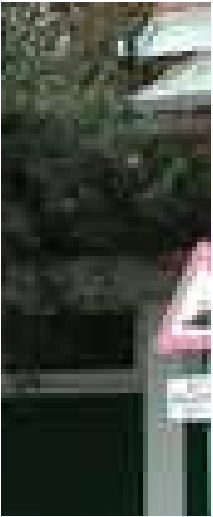
\includegraphics[height=1.7in]{../figures/examplePicture-crop.pdf} \label{fig:examplePicture}}
  \;
  \subfigure[features]{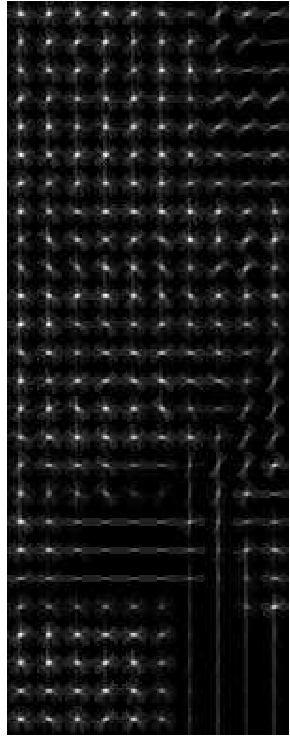
\includegraphics[height=1.7in]{../figures/exampleFeature-crop.pdf} \label{fig:exampleFeature}}
  \caption{ \ref{fig:examplePicture} picture No 200 and \ref{fig:exampleFeature} features extracted form it, using Piotr's toolbox (http://vision.ucsd.edu/~pdollar/toolbox/doc/index.html) %TODO where put this reference
  }
\end{figure}

\subsection{Data analysis and preparation}
  Features first two dimensions $26\times10$ of features for particular image correspond to the position of image form where those features were extracted and in the third dimension corresponds to the direction of edges in that part of image. White color and big number indicates that there is the edge, see \ref{fig:examplePicture} and \ref{fig:exampleFeature}. Values of features are between $0$ and $0.2$ and normalization doesn't change them much. 
  \begin{figure}[!h]
  \center
  \subfigure[original data]{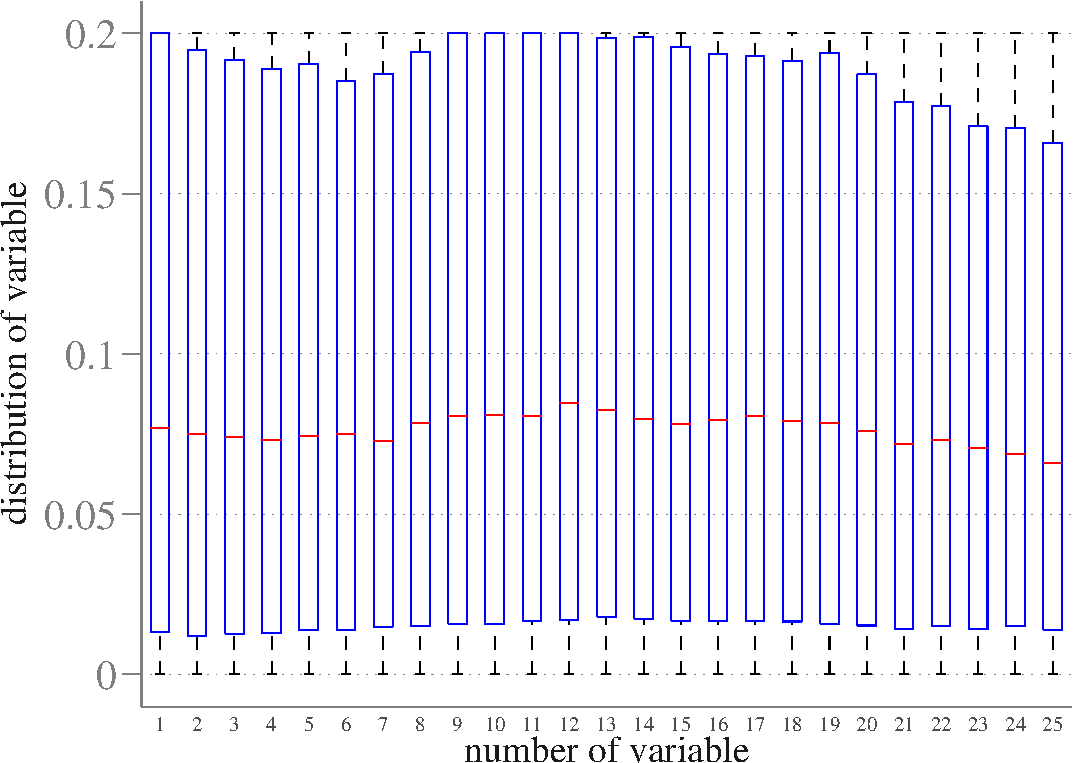
\includegraphics[height=1.8in]{../figures/boxplot1-crop.pdf} \label{fig:boxplot1}}
  \;
  \subfigure[after normalization]{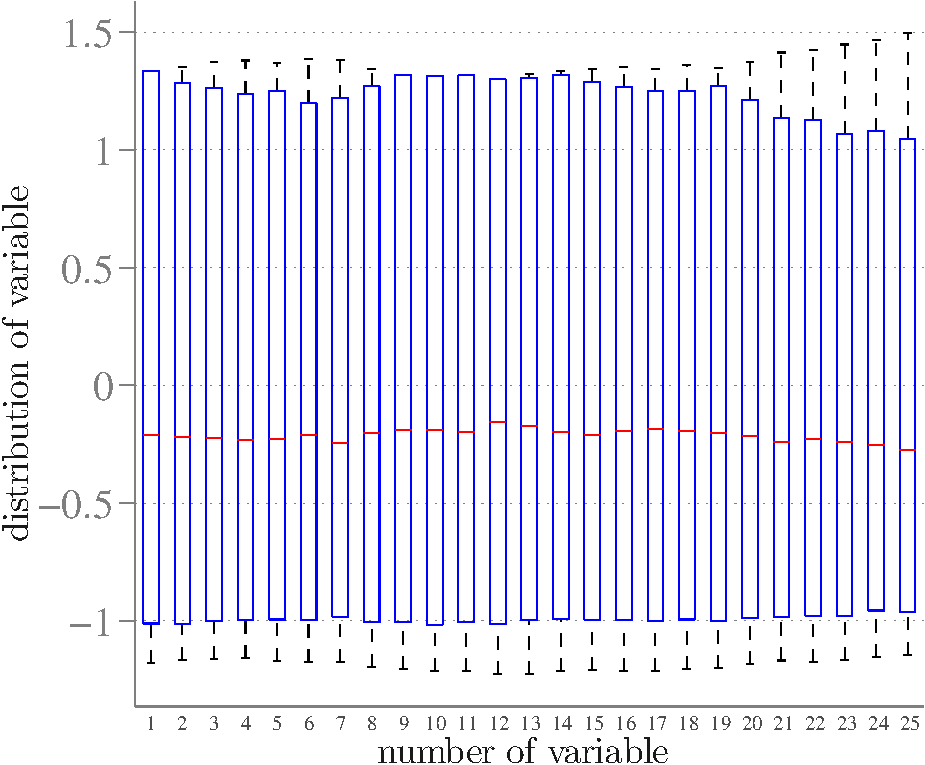
\includegraphics[height=1.8in]{../figures/boxplot2-crop.pdf} \label{fig:boxplot2}}
  \caption{Boxplots of part of the data before \ref{fig:boxplot1} and after \ref{fig:boxplot2} normalization. Rest of the data looks similar.}
\end{figure}
  
  Since there are $9360$ numbers for one picture using all of them may cause overfitting. We calculated correlation of them with output and we obtained picture of abstract person, see \ref{fig:correlation}.
  Also on figure \ref{fig:correlations} we can see that there are regions and gradient more and less important for this task and they have shape of a person. Values of correlation were between $-0.37$ and $0.37$
  \begin{figure}[t]
    \center
    \subfigure[Absolute value of correlation for different directions of gradient]{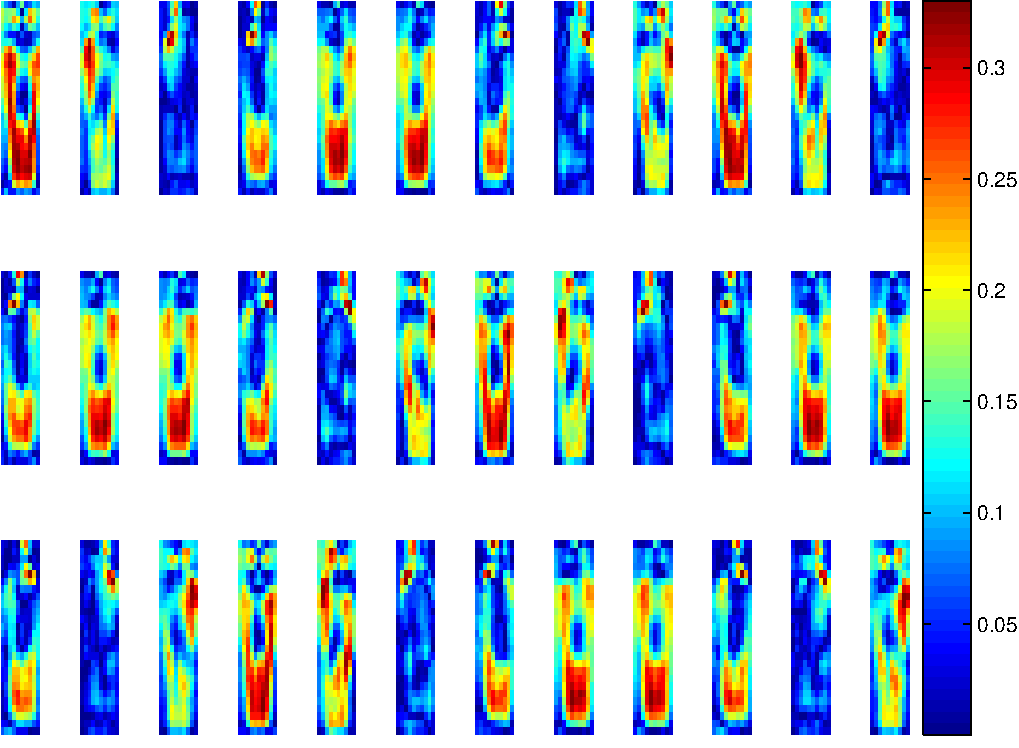
\includegraphics[height=1.7in]{../figures/absoluteCorelation-crop.pdf} \label{fig:correlations}}
      \;\;\;
    \subfigure[positive correlation]{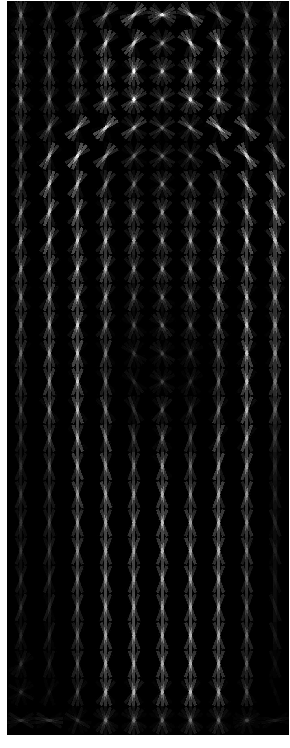
\includegraphics[height=1.7in]		{../figures/averagePerson-crop.pdf} \label{fig:correlation}}
    \caption{Absolute value \ref{fig:correlations} and only positive part \ref{fig:correlation} of correlation, plotted as a feature. It may be good to not use the deep blue data.}
  \end{figure}
   
% TODO: test matrices descriptions.

\section{Applied methods}
We applied many methods for this task, for most of them we used existing libraries. To check which method is better we were were plotting doing cross-validation and then taking predictions into one big vector and passing it as predictions to function \verb+evaluateMultipleMethods+, which was given to us together with data. 

\subsection{Penalized logistic regression}
We started with the the simplest (penalized) logistic regression. We tied different penalties ($\lambda$) and different number of features. We were setting parameter $threshold$ to some value between $0$ and $0.37$, and taking only the part of features which are more correlated to output than $threshold$ (in absolute value). The best True Position Rate we got for this model was $0.231$ for $threshold = 0.1$ and $\lambda = 0.8$. Taking more data wasn't changing TPR and changing ROC curve slightly.  %TODO revrite this, picture is almost write :/ or maby 0.700 is good assuption

  \begin{figure}[h]
    \center
    \subfigure[ROC curves for linear model and for random assignment.]{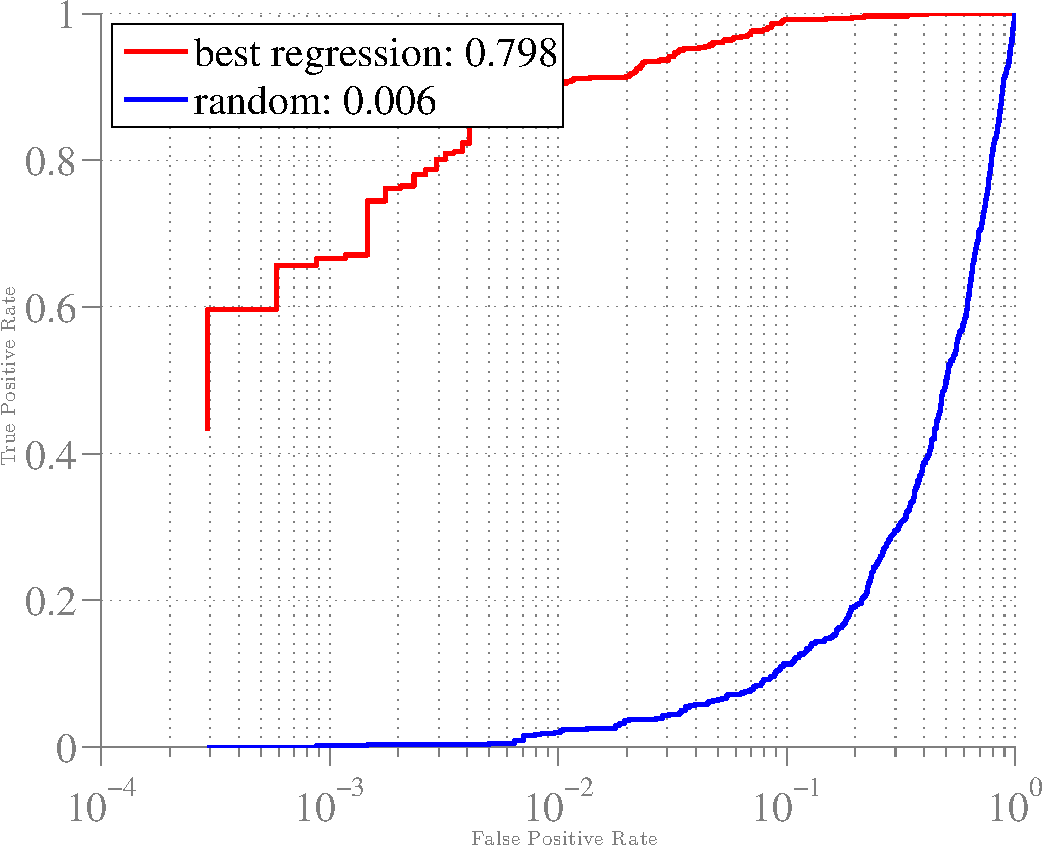
\includegraphics[height=1.7in]{../figures/ROClinear-crop.pdf} \label{fig:ROClinear}}
    \caption{ROC curves for different models}
  \end{figure}

\subsection{SVM}

\subsection{Neural Network}

\subsection{Random Forest}



\end{document}
